% id: 0231
% book: RPM 중3-2 수학 · 02 삼각비의 활용
% section: 중단원 마무리하기
% figure: crop:fig-0231.png
% answer: ⑤
% answer_source: 답지
% variant_level: 0 (원본 전사)
% 이 파일은 build.mjs 가 items.json 에서 만든다. 고칠 때는 items.json 을 고친다.
\noindent\begin{minipage}[t]{0.58\linewidth}\vspace{0pt}\raggedright 오른쪽 그림의 $\triangle\pt{ABC}$에서 $\angle\pt{B}=75^\circ$, $\angle\pt{C}=45^\circ$, $\seg{AB}=20\mkern3mu \mathrm{cm}$일 때, $x+y$의 값은?\end{minipage}\hfill\begin{minipage}[t]{0.4\linewidth}\vspace{0pt}\centering \setlength{\dmfigw}{92.3pt}\ifdim\dmfigw>\linewidth\setlength{\dmfigw}{\linewidth}\fi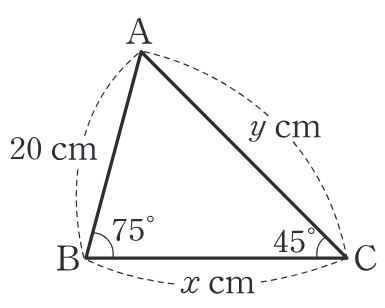
\includegraphics[width=\dmfigw]{figures/fig-0231.png}\end{minipage}\par
\begin{choicesv}{$10(1+\sqrt{2})$}{$10(1+\sqrt{3})$}{$10(1+\sqrt{2}+\sqrt{3})$}{$10(1+\sqrt{2}+\sqrt{5})$}{$10(1+\sqrt{3}+\sqrt{6})$}\end{choicesv}
